\documentclass[../main.tex]{subfiles}

\begin{document}

\section{Determinación de la carga del viento}

El primer paso para éste análisis de viento. Esto lo hacemos a partir del método
explicado en el capitulo 5 del reglamento CIRSOC 102. 

Primero, obtenemos la \textbf{velocidad básica del viento} a partir de la figura
1A, el \textbf{factor de direccionalidad} a partir de la Tabla 6, el \textbf{factor}
\textbf{de importancia} para un edificio Categoría II a partir de la tabla y 
un factor topográfico a partir del artículo 5.7. 
Resumiendo, obtenemos:

\begin{align*}
  V &= \SI{50}{m / s} \\[5pt]
  k_d &= 0.85 \\[5pt]
  I &= 1 \\[5pt]
  K_{zt} &= 1
.\end{align*}

Luego a partir de la Tabla 5 determinamos lo siguiente:

% Table generated by Excel2LaTeX from sheet 'Integrador'
\begin{table}[htbp]
  \centering
    \begin{tabular}{|l|c|}
    \hline
    Categoría de exposición & B \bigstrut\\
    \hline
    $\alpha$     & 7.00 \bigstrut\\
    \hline
    zg [m] & 366.00 \bigstrut\\
    \hline
    \end{tabular}%
  \label{tab:addlabel}%
\end{table}%

Obtenemos el coeficiente de exposición para la presión dinámica según la altura:

\begin{align*}
  k_z &= 2.01 * ( z / z_g)^{2 / \alpha} \hspace{0.25cm} \xrightarrow{\hspace*{0.5cm}} \hspace{0.1cm} \text{para } \SI{5}{m}\leq z\leq z_g \\[5pt]
  k_z &= 2.01 * (5 / z_g)^{2 / \alpha} \hspace{0.25cm} \xrightarrow{\hspace*{0.5cm}} \hspace{0.1cm} \text{para } z \leq \SI{5}{m}
.\end{align*}

Podemos formular la siguiente tabla:

% Table generated by Excel2LaTeX from sheet 'Integrador'
\begin{table}[htbp]
  \centering
  \caption{Coeficiente de exposición $q_z$}
    \begin{tabular}{|l|c|c|c|}
    \hline
    \rowcolor[rgb]{ .851,  .882,  .949} z                [m] & \cellcolor[rgb]{ 1,  1,  1}0.00 & \cellcolor[rgb]{ 1,  1,  1}3.73 & \cellcolor[rgb]{ 1,  1,  1}7.45 \bigstrut\\
    \hline
    \rowcolor[rgb]{ .851,  .882,  .949} Kz    & \cellcolor[rgb]{ 1,  1,  1}0.59 & \cellcolor[rgb]{ 1,  1,  1}0.59 & \cellcolor[rgb]{ 1,  1,  1}0.66 \bigstrut\\
    \hline
    \rowcolor[rgb]{ .851,  .882,  .949} qz    [KN/m²] & \cellcolor[rgb]{ 1,  1,  1}768.55 & \cellcolor[rgb]{ 1,  1,  1}768.55 & \cellcolor[rgb]{ 1,  1,  1}859.73 \bigstrut\\
    \hline
    \end{tabular}%
\end{table}%

Luego, obtenemos el factor de ráfaga de la siguiente forma:

\begin{align*}
  G = 0.85
.\end{align*}

\subsection{Clasificación de cerramiento}

Siguiendo el artículo 5.9, obtenemos el área total de aberturas en una pared $A_o$,
el área total de la misma pared  $A_g$, la suma de las áreas de abertura en la 
envolvente del edificio $A_{oi}$ y la suma de las áreas totales de la 
envolvente del edifcio $A_{gi}$. Con esto verifciamos:

\begin{align*}
  A_g &= \SI{126.3}{m^2} \\[5pt]
  A_o &= \SI{21.6}{m^2}
.\end{align*}

Vemos que $\SI{101.02}{m^2}\leq  A_o$, entonces procedemos con la verificación de
un edificio parcialmente cerrado.
Para esto obtenemos:

\begin{align*}
  A_g &= \SI{126.3}{m^2} \\[5pt]
  A_o &= \SI{21.6}{m^2} \\[5pt]
  A_{oi} &= \SI{7.2}{m^2} \\[5pt]
  A_{gi} &= \SI{71.7}{m^2}
.\end{align*}

Con esto también verificamos que:

\begin{align*}
  \SI{7.92}{m^2} &\leq  A_o \hspace{0.25cm} \xrightarrow{\hspace*{0.5cm}} \hspace{0.1cm} \text{Cumple}\\[5pt] 
  \SI{0.4}{m^2} &\leq A_o \hspace{0.25cm} \xrightarrow{\hspace*{0.5cm}} \hspace{0.1cm} \text{Cumple} \\[5pt] 
  \SI{0.1}{m^2} &\geq 0.2 \hspace{0.25cm} \xrightarrow{\hspace*{0.5cm}} \hspace{0.1cm} \text{\textbf{No cumple}} 
.\end{align*}

Entonces determinamos que tenemos un \textbf{edificio cerrado}.

\subsection{Coeficente de presión interna}

Se determina el valor del coeficiente de presión interna $Gcpi$ a partir de la 
tabla 7, que nos da:

\begin{align*}
  Gcpi = \pm 0.18
.\end{align*}

Por último, obteniendo el valor de $C_p$, podemos desarrollar la siguiente
tabla:

\begin{figure}[ht]
  \centering
  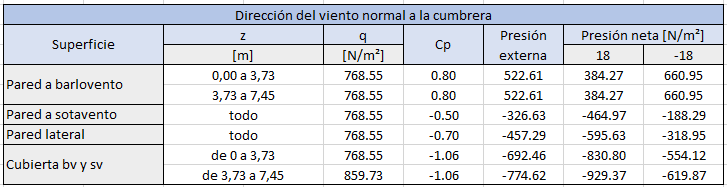
\includegraphics[width=1\textwidth]{../images/normal_cumbrera}
  \label{fig:normal_cumbrera}
\end{figure}

\begin{figure}[ht]
  \centering
  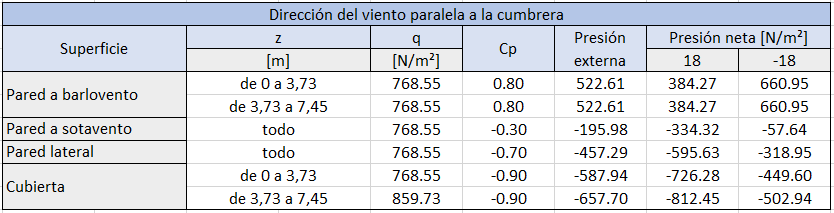
\includegraphics[width=1\textwidth]{../images/paralelo_cumbrera}
\end{figure}

\clearpage

En resumen, entonces podemos obtener las siguientes cargas de viento:

% Table generated by Excel2LaTeX from sheet 'Integrador'
\begin{table}[htbp]
  \centering
    \begin{tabular}{|c|c|cc|cc|}
    \hline
    \multirow{2}[2]{*}{Elemento} & \cellcolor[rgb]{ .851,  .882,  .949}Separación & \multicolumn{2}{c|}{\cellcolor[rgb]{ .851,  .882,  .949}Presión de diseño} & \multicolumn{2}{c|}{\cellcolor[rgb]{ .851,  .882,  .949}Carga de viento} \bigstrut[t]\\
          & \cellcolor[rgb]{ .929,  .929,  .929}[m] & \multicolumn{2}{c|}{\cellcolor[rgb]{ .929,  .929,  .929}[KN/m²]} & \multicolumn{2}{c|}{\cellcolor[rgb]{ .929,  .929,  .929}[KN/m]} \bigstrut[b]\\
    \hline
    \rowcolor[rgb]{ .929,  .929,  .929} Correa & \cellcolor[rgb]{ 1,  1,  1}1.00 & \multicolumn{2}{c|}{\cellcolor[rgb]{ 1,  1,  1}-0.93} & \multicolumn{2}{c|}{\cellcolor[rgb]{ 1,  1,  1}-0.93} \bigstrut[t]\\
    \rowcolor[rgb]{ .929,  .929,  .929} Viga  & \cellcolor[rgb]{ 1,  1,  1}4.20 & \multicolumn{2}{c|}{\cellcolor[rgb]{ 1,  1,  1}-0.93} & \multicolumn{2}{c|}{\cellcolor[rgb]{ 1,  1,  1}-3.90} \bigstrut[b]\\
    \hline
    \end{tabular}%
  \label{tab:addlabel}%
\end{table}%




\end{document}
